\chapter{K"unstliche neuronale Netze}
{
K"unstliche Intelligenz l"asst sich mit einem K"unstlichen Neuronalen Netz (KNN) realisieren. KNNs basieren auf dem Vorbild des biologischen neuronalen Netz des Gehirns.
\cite{Breitner} schreibt dazu:
\begin{quote}{\glqq}Die biologischen Vorg"ange des menschlichen Denkens und Lernens (Aktivierung von Neuronen, chemische Ver"anderung von Synapsen usw.) werden, so gut wie m"oglich, mathematisch beschrieben und in Software oder Hardware modelliert.{\grqq}\end{quote}
KNNs bestehen also aus einem Satz von Algorithmen, welche Daten interpretieren. Diese Eingangsdaten sind numerisch und m"ussen meist durch Umwandlung der originalen Daten (z.B. Bilder, Text oder Musik) geschaffen werden. Sie sind dazu entwickelt anhand von Mustererkennung Daten eigenst"andig zu Gruppieren, vorgegebenen Klassen zu zuordnen oder den weiteren Verlauf vorherzusagen.

Das Training eines KNNs l"asst sich in zwei Kategorien unterteilen: das "uberwachte Lernen und das un"uberwachte Lernen. Beim "uberwachten lernen werden dem Netz Eingangs- und Ausgangsdaten gegeben anhand dessen das Netz den Zusammenhang erlernt und sp"ater in der Lage ist neue Daten entsprechend zu klassifizieren oder die n"achsten Ausgabe vorherzusagen. Beim un"uberwachten Lernen erh"alt das Netz lediglich Eingangsdaten und lernt diese anhand von "Ahnlichkeiten  zu gruppieren.

Es gibt verschiedene Arten von K"unstlichen Neuronalen Netzen und in den folgenden Abschnitten werden drei von ihnen erkl"art.


\section{Feedforward Netzwerke}
Ein Feedforward Netzwerk besteht aus Layern und Neuronen. Die Neuronen sind f"ur die Berechnungen der Ausgabe zust"andig, w"ahrend die Layer den Aufbau des Netzes bestimmen. Abbildung 2.1 zeigt einen m"oglichen Aufbau eines k"unstliches Neurons.
\renewcommand{\figurename}{Abb.}
\begin{figure}[htp]
\centering
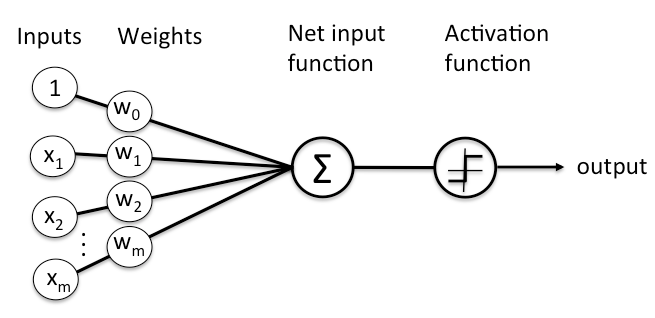
\includegraphics[width=0.60\textwidth]{pictures/perceptron_node.png}
\caption[Feedforward Neuron]{m"ogliches Aussehen eines Feedforward Neurons (Quelle: \cite{DL4Jimg1})}
\end{figure}
Dieses Neuron besteht aus 1 bis x\textsubscript{m} Eing"angen (Inputs) mit Gewichten (Weights), einer Eingangsfunktion (Net input function), einer Aktivierungsfunktion (Activation function) und einem Ausgang (Outputs). Die zu verarbeiteten Daten werden an die Eing"ange gelegt, durch die zugeh"origen Gewichte verst"arkt oder abgeschw"acht und anschlie{\ss}end durch die Eingangsfunktion aufsummiert. Die entstandene Summe wird dann an die Aktivierungsfunktion "ubergeben, welche das Ergebnis dieses Neurons festlegt.

Ein Layer besteht aus einer Reihe von Neuronen beliebiger Anzahl. Ein k"unstliches neuronales Netz setze sich aus einem Input Layer, einem Output Layer und beliebig vielen Hidden Layern zusammen. Hat ein Netz mehr als ein Hidden Layer so wird es auch als Deep Learning Netz bezeichnet.
\renewcommand{\figurename}{Abb.}
\begin{figure}[htp]
\centering
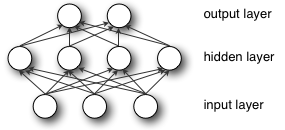
\includegraphics[width=0.50\textwidth]{pictures/mlp.png}
\caption[Aufbau eines Feedforward Netzes]{Aufbau eines Feedforward Netzes (Quelle: \cite{DL4Jimg1})} 
\end{figure}
Abbildung 2.2 zeigt ein Feedforward Netzwerk. Bei diesem Netz besitzt das Input Layer drei Neuronen, das Hidden Layer hat vier und das Output Layer hat zwei Neuronen. Die Ergebnisse des Input und Hidden Layers dienen dem nachfolgenden Layer als Eingang. Die Eing"ange des Input Layers und der Ausgang des Output Layers sind hier nicht dargestellt, da der Fokus auf der inneren Verkn"upfung liegen soll. Jedes Neuron hat hier so viel Ausg"ange wie die Anzahl der Neuronen im folgenden Layer und ist somit vollst"andig verkn"upft. Dies muss nicht immer der Fall sein, doch auf diesen Sonderfall soll hier nicht weiter eingegangen werden.


\subsection{Training durch Backpropagation}
Ein neuronales Netz kann anhand von Trainingsdaten eine Funktion erlernen, indem es die Gewichte ver"andert. Um sinnvolle Ergebnisse zu erhalten m"ussen die Gewichte solange angepasst werden, bis der Fehler zwischen Netzausgabe und tats"achlichen Ausgabewert am kleinsten ist. Dies wird mit Hilfe der Backpropagation gemacht, indem R"uckw"arts vom Fehler "uber die Ausg"ange, die Gewichte und die Eing"ange der verschiedenen Layer ein Zusammenhang zwischen Fehlergr"o{\ss}e und einzelnen Gewichtseinstellungen hergestellt wird. F"ur die Bestimmung der ben"otigten Gewichten benutzt man Optimierungsfunktionen. Eine weitverbreitete Optimierungsfunktion hei{\ss}t Gradient Descent. Sie beschreibt das Verh"altnis des Fehlers zu einem einzelnen Gewicht und wie sich der Fehler ver"andert wenn das Gewicht angepasst wird.

Das Ziel ist m"oglichst schnell den Punkt zu erreichen an dem der Fehler am kleinsten ist. Um dies zu erreichen wiederholt das Netz so oft wie n"otig die folgenden Schritte: Ergebnis anhand der aktuellen Gewichte bestimmen, Fehler messen, Gewichte aktualisieren.


\section{Recurrent Netzwerke}
Recurrent Neuronal Networks (RNN) betrachten im Gegensatz zu Feedforward Netzwerken nicht nur die aktuellen Eingangsdaten sondern auch die vorhergegangenen. Sie besitzen daher zwei Eingangsgr"o{\ss}en, n"amlich die gerade angelegten und die zur"uckgeleiteten aus dem vorherigen Zeitschritt.
\renewcommand{\figurename}{Abb.}
\begin{figure}[htp]
%%\begin{floatingfigure}[r]{textwidth}
\centering
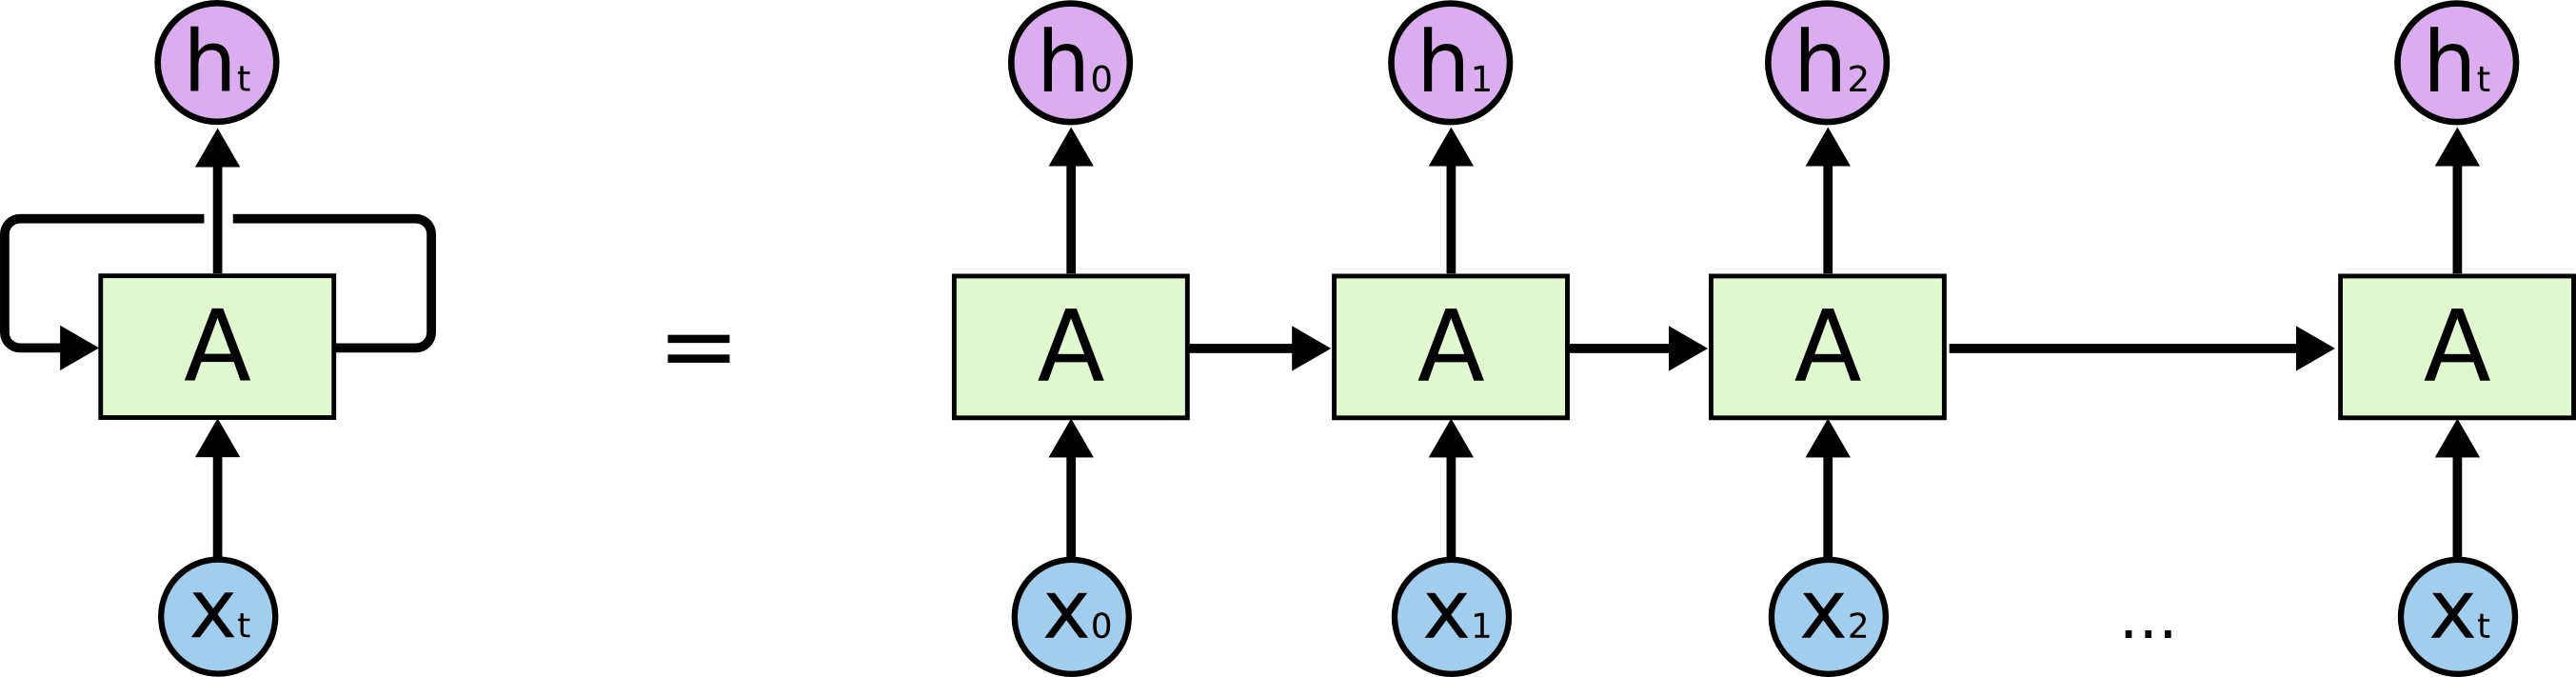
\includegraphics[width=0.60\textwidth]{pictures/RNN-unrolled.png}
\caption[RNN Neuron]{vereinfachte Darstellung eines RNN Neurons (Quelle: \cite{OlahImg})}
%%\end{floatingfigure} 
\end{figure}
Abbildung 2.3 zeigt links eine vereinfachte Darstellung eines RNN Neurons mit R"uckf"uhrung, aber ohne dargestellte Gewichte oder Aktivierungsfunktion. Rechts ist das Ganze als zeitlicher Verlauf dargestellt. Im ersten Zeitschritt wird x\textsubscript{0} an den Eingang gelegt und h\textsubscript{0} als Ergebnis berechnet. Au{\ss}erdem f"uhrt ein Pfeil zum Neuron im zweiten Zeitschritt und dient dort als zweiter Eingang. Das Ergebnis, das ein Neuron liefert ist also immer vom vorherigen abh"angig. Man bezeichnet dies auch als Ged"achtnis des Netzes. Einem Netz ein Ged"achtnis zu geben macht immer dann Sinn, wenn die Eingangsdaten eine Sequenz bilden und nicht komplett unabh"angig von einander sind. Im Gegensatz zu den Feedforward Netzen k"onnen Recurrent Netzwerke Sequenzen erfassen und sie zur Erzeugung ihrer Ausgaben nutzen. Dies ist zum Beispiel bei der automatischen Textgenerierung hilfreich, wo ein folgender Buchstabe immer vom vorherigen abh"angt und nicht willk"urlich gew"ahlt werden kann. Ein RNN ist in der Lage gezielt auf ein q ein u folgen zu lassen um sinnvolle W"orter zu bilden, ein Feedforward Netzwerk kann das nicht.

\subsection{Training durch Backpropagation Through Time}
Da bei Recurrent Netzen das Ergebnis und somit der Fehler nicht nur vom aktuellen Zeitschritt abh"angt, muss auch die Backpropagation erweitert werden um sinnvoll arbeiten zu k"onnen. Backpropagation Through Time (BPTT) erg"anzt die normale Backpropagation um den Faktor Zeit, so dass ein Einfluss auf den Fehler von einem Gewicht aus fr"uheren Schritten ermittelt werden kann. Abbildung 2.4 soll diesen Vorgang verdeutlichen. 
\renewcommand{\figurename}{Abb.}
\begin{figure}[hb]
\centering
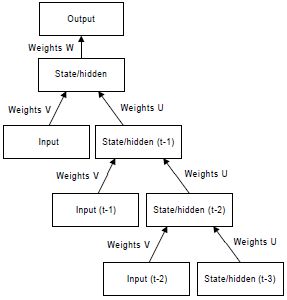
\includegraphics[width=0.65\textwidth]{pictures/bptt_cut.png}
\caption[BPTT]{entrolltes RNN f"ur BPTT (Quelle: \cite{BPTT})}
\end{figure}
Sie zeigt ein Recurrent Netz das um drei Zeitschritte entrollt wurde indem Komponenten dupliziert wurden. Dadurch l"osen sich die R"uckf"uhrungen auf und das Netzwerk verh"alt sich wie ein Feedforward Netz. Der Einfluss jedes Gewichts kann nun anteilig berechnet und anschlie{\ss}end summiert werden, so dass ein einzelner Wert je Gewicht f"ur die Anpassung ermittelt wird.

Dieses Verfahren ben"otigt nat"urlich mehr Speicher, da alle vorherigen Zust"ande und Daten f"ur eine bestimme Anzahl an Zeitschritten gespeichert werden m"ussen.


\subsection{Problem der verschwindenden und explodierenden Gradienten}
Der Gradient stellt die Ver"anderung aller Gewichte in Bezug auf Ver"anderung im Fehler dar. Wenn der Gradient unbekannt ist, ist eine Ver"anderung an den Gewichten zur Verkleinerung des Fehlers nicht m"oglich und das Netz ist nicht in der Lage zu lernen. Zu unbekannten Gradienten kann es kommen, da Informationen die durch ein Deep Netz flie{\ss}en vielfach multipliziert werden. Multipliziert man einen Betrag regelm"a{\ss}ig mit einem Wert knapp gr"o{\ss}er 1 kann das Ergebnis unmessbar gro{\ss} werde und in diesem Fall spricht man von einem explodierenden Gradienten. Umgekehrt f"uhrt eine wiederholte Multiplikation eines Betrages mit einem Wert kleiner als 1 zu einem sehr kleinem Ergebnis. Der Wert kann so klein werden, dass er von einem Netz nicht mehr gelernt werden kann. Hier spricht man von einem verschwindenden Gradienten.

Das Problem der explodierenden Gradienten l"asst sich durch eine sinnvolle Obergrenze beheben. Bei den verschwindenden Gradienten sieht eine L"osung wesentlich schwieriger aus und dieses Thema ist noch immer Gegenstand der Forschung.


\subsection{Problem der Langzeit-Abh"angigkeiten}
Wie bereits erw"ahnt sind RNNs in der Lage Sequenzen zu erkennen und mit Abh"angigkeiten zu arbeiten, doch diese F"ahigkeit ist leider begrenzt. Besteht nur eine kleine zeitliche L"ucke zwischen den von einander abh"angigen Daten, ist ein RNN in der Lage diesen Zusammenhang zu erkennen und die richtigen Schl"usse zu ziehen. Wird der zeitliche Abstand zwischen Eingabe der Daten und dem Zeitpunkt an dem sie f"ur ein Ergebnis ben"otigt werden jedoch sehr gro{\ss} kann ein RNN diesen Zusammenhang nicht mehr herstellen. Als Beispiel gibt \cite{Olah} in seinem Artikel ein Sprach-Model an, welches das n"achste Wort abh"angig vom Vorherigen vorhersagt. Ein RNN ist in der Lage im Satz {\glqq}Die Wolken sind im Himmel.{\grqq} das letzte Wort vorauszusagen, da der Abstand von Himmel und Wolken sehr klein ist. Im Text {\glqq}Ich bin in Frankreich aufgewachsen. ... Ich spreche flie{\ss}end franz"osisch.{\grqq} kann der Abstand zum letzten Wort aber sehr gro{\ss} sein und die vorherigen W"orter lassen lediglich den Schluss zu das eine Sprache folgen muss. Denn Kontext, dass es sich sehr wahrscheinlich um franz"osisch handelt, erh"alt man nur durch den ersten Satz. Ein RNN kann sich aber keinen ganzen Text merken und somit hier den Zusammenhang von Frankreich und franz"osisch nicht lernen.

Um das Problem der Langzeit-Abh"angigkeiten zu l"osen, benutzt man Long Short-Term Memory Netze.


\section{Long Short-Term Memory Netze}
Long Short-Term Memory (LSTM) Netze sind eine besondere Art von Recurrent Netzwerken, die mit Langzeit-Abh"angigkeiten arbeiten k"onnen. Sie wurden so entworfen, dass sie speziell dieses Problem l"osen, denn Informationen "uber einen langen Zeitraum zu speichern ist ihr Standardverhalten und nicht etwas was m"uhsam erlernt werden muss. Sie bestehen aus Speicherzellen, in die Informationen geschrieben und wieder herausgelesen werden k"onnen. Mit Hilfe von sogenannten Gates, die ge"offnet oder geschlossen werden, entscheidet eine Zelle was gespeichert wird und wann ein Auslesen, Reinschreiben und L"oschen erlaubt ist. Diese Gates sind analog und durch eine Sigmoid-Funktion implementiert, so dass sich ein Bereich von 0 bis 1 ergibt. (Analog hat den Vorteil gegen"uber digital dass es differenzierbar ist und somit f"ur die Backpropagation geeignet.)
\renewcommand{\figurename}{Abb.}
\begin{figure}[htb]
\centering
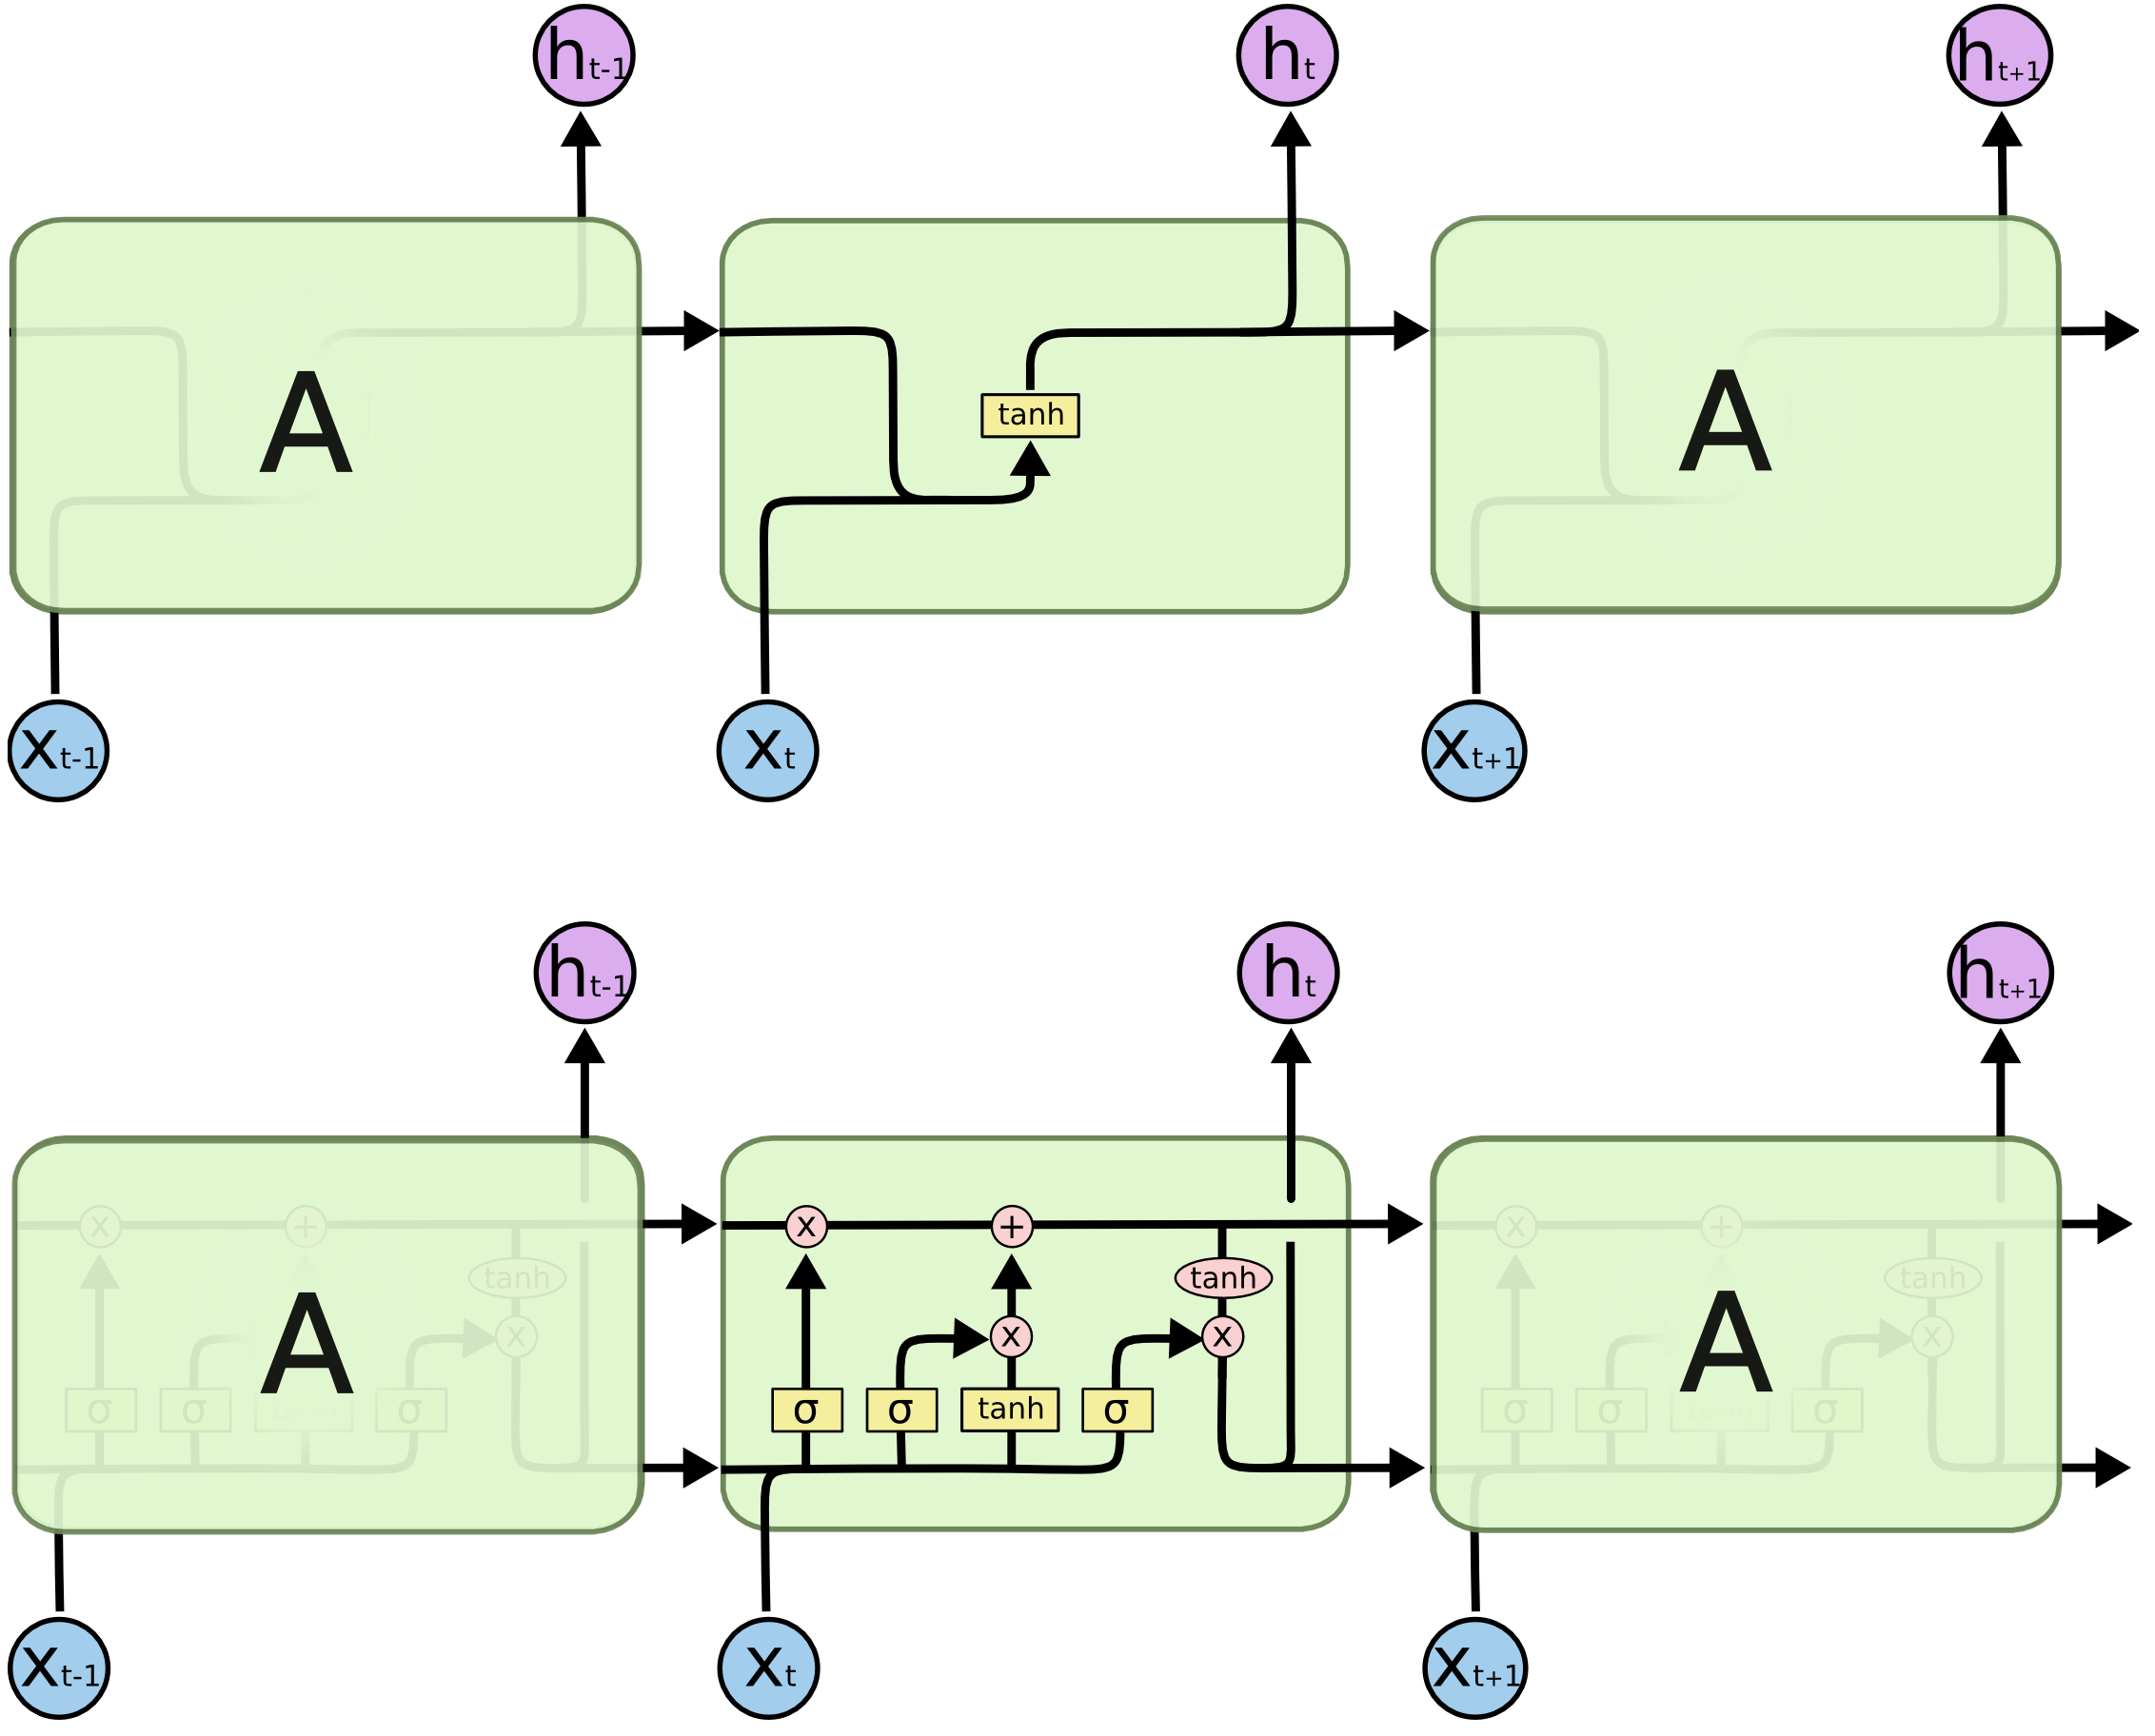
\includegraphics[width=0.75\textwidth]{pictures/SRN-LSTM-chain.png}
\caption[Vergleich RNN und LSTM]{Vergleich RNN und LSTM (Quelle: \cite{OlahImg})}
\end{figure}
Genau wie die Eing"ange bei den Feedforward und Recurrent Netzen besitzen die Gates Gewichte. Diese Gewichte werden ebenfalls w"ahrend des Lernprozesses angepasst, so dass die Zelle lernt wann Daten eingelassen, ausgelesen oder gel"oscht werden m"ussen.

Abbildung 2.5 zeigt zum Vergleich oben ein simples Recurrent Netz und unten ein LSTM Netz. Beide sind "uber drei Zeitschritte dargestellt, wobei der zweite Schritt jeweils ihr Innenleben wiedergibt. W"ahrend beim RNN eine simple Struktur mit nur einer Funktion (gelber Kasten in der Abbildung) f"ur das Ergebnis verantwortlich ist, benutzt ein LSTM vier Funktionen. Wie diese Funktionen mit einander agieren und zu einem Ergebnis kommen wird im n"achsten Abschnitt Schrittweise erkl"art.


\subsection{Aufbau einer Speicherzelle}
\subsubsection{Zellzustand}
\begin{wrapfigure}{r}{0.45\textwidth}
  \vspace{-30pt}
  \begin{center}
    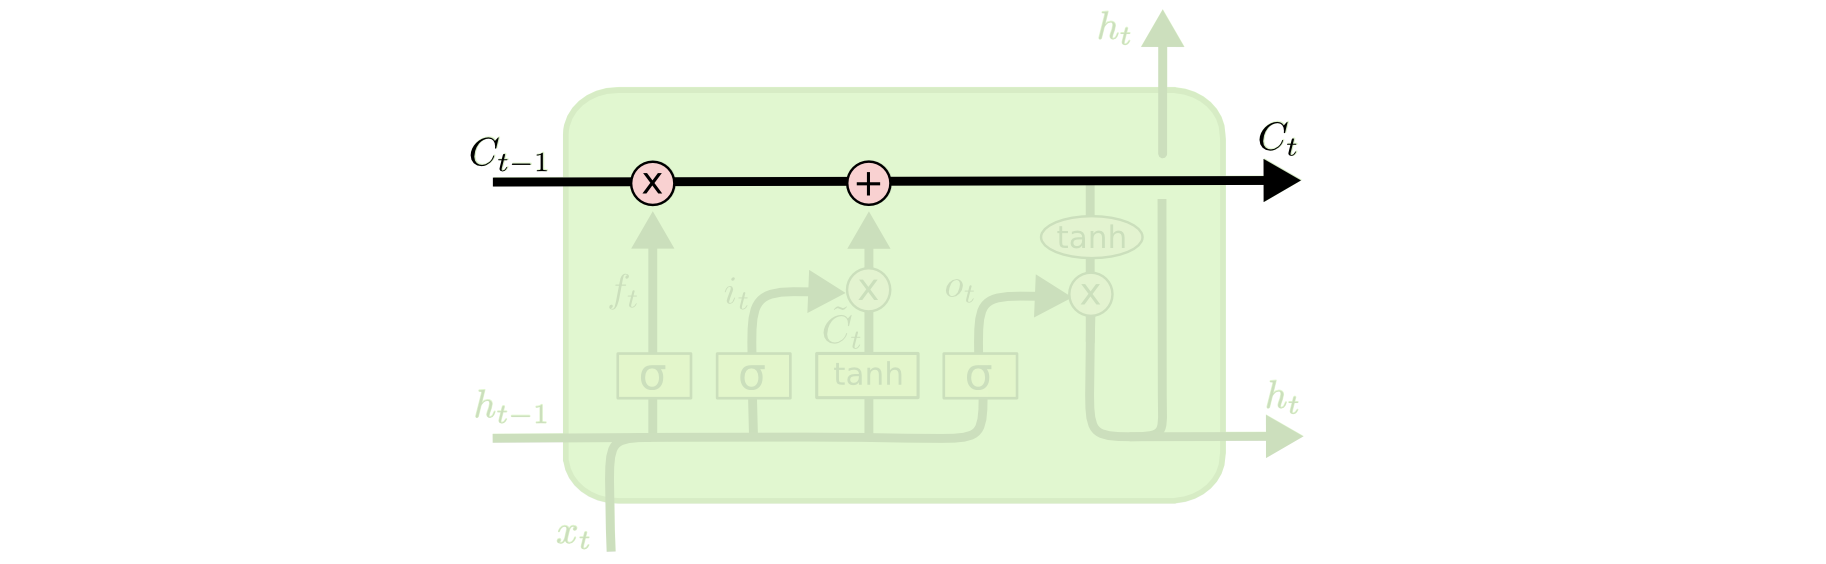
\includegraphics[width=0.45\textwidth]{pictures/LSTM3-C-line.png}
  \end{center}
  \vspace{-20pt}
  \caption[LSTM Zellzustand]{LSTM Zellzustand (Quelle: \cite{OlahImg})}
\vspace{-10pt}
\end{wrapfigure}
Der Zellzustand ist der eigentliche Speicherort oder das Ged"achtnis des LSTM. Abbildung 2.6 zeigt den Verlauf durch eine Speicherzelle. Links wird der Zellzustand vom vorherigen Zeitschritt "ubernommen und rechts an den n"achsten weitergegeben. In der Mitte sind zwei Operation, die den Zustand w"ahrend dieses Zeitschrittes ver"andern k"onnen. Welche Aufgabe sie haben folgt im Abschnitt Zellzustands Update.

\subsubsection{Forget Gate}
\begin{wrapfigure}{r}{0.45\textwidth}
  \vspace{-30pt}
  \begin{center}
    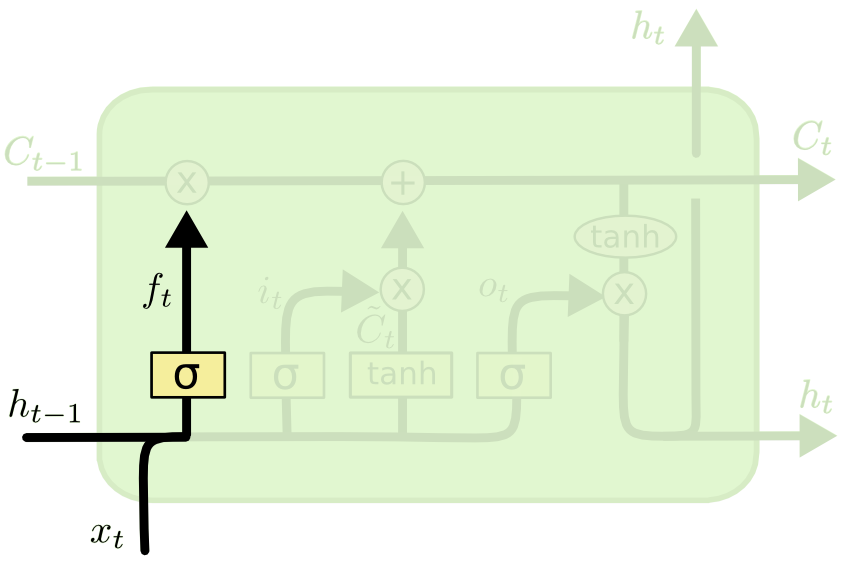
\includegraphics[width=0.45\textwidth]{pictures/LSTM3-focus-f_cut.png}
  \end{center}
  \vspace{-20pt}
  \caption[LSTM: Forget Gate]{Forget Gate (Quelle: \cite{OlahImg})}
\vspace{-10pt}
\end{wrapfigure}
Das Forget Gate entscheidet mit Hilfe der Sigmoid-Funktion welche Informationen gel"oscht werden. Es sieht sich den alten Ausgang h\textsubscript{t-1} und den neuen Eingang x\textsubscript{t} an und gibt f"ur jede Information im Zellzustand C\textsubscript{t-1} einen Wert zwischen 0 und 1 an. Eine 1 bedeutet behalte es und eine 0 vergiss bzw. l"osche es.

Der Grund f"ur das Vorhandensein einer Vergissfunktion in einem Baustein, der die Aufgabe hat sich Sachen zu merken, liegt darin dass es manchmal sinnvoll sein kann Dinge zu vergessen. Zum Beispiel kann mit ihrer Hilfe die Speicherzelle zur"uckgesetzt werden, wenn bekannt ist dass die folgenden Daten in keinem Zusammenhang zu den vorherigen stehen.

\subsubsection{Eingang}
\begin{wrapfigure}{r}{0.45\textwidth}
  \vspace{-30pt}
  \begin{center}
    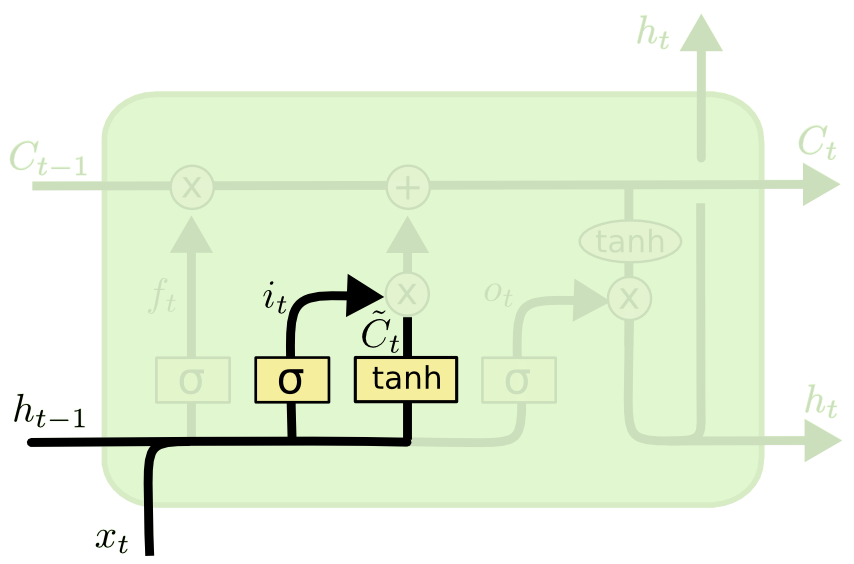
\includegraphics[width=0.45\textwidth]{pictures/LSTM3-focus-i_cut.png}
  \end{center}
  \vspace{-20pt}
  \caption[LSTM: Eingangsgate]{Eingangsgate (Quelle: \cite{OlahImg})}
\vspace{-10pt}
\end{wrapfigure}
Die Entscheidung, welche Daten gespeichert werden sollen, besteht aus zwei Teilen. Das Eingangsgate ist ebenfalls eine Sigmoid-Funktion und liefert ein Ergebnis zwischen 0 und 1. Sie entscheidet welche Daten zum Zellzustand wie stark durchgelassen werden. Au{\ss}erdem bereitet eine tanh-Funktion die Daten so auf, dass sie im Zellzustand gespeichert werden k"onnen.

\subsubsection{Zellzustands Update}
\begin{wrapfigure}{r}{0.45\textwidth}
  \vspace{-30pt}
  \begin{center}
    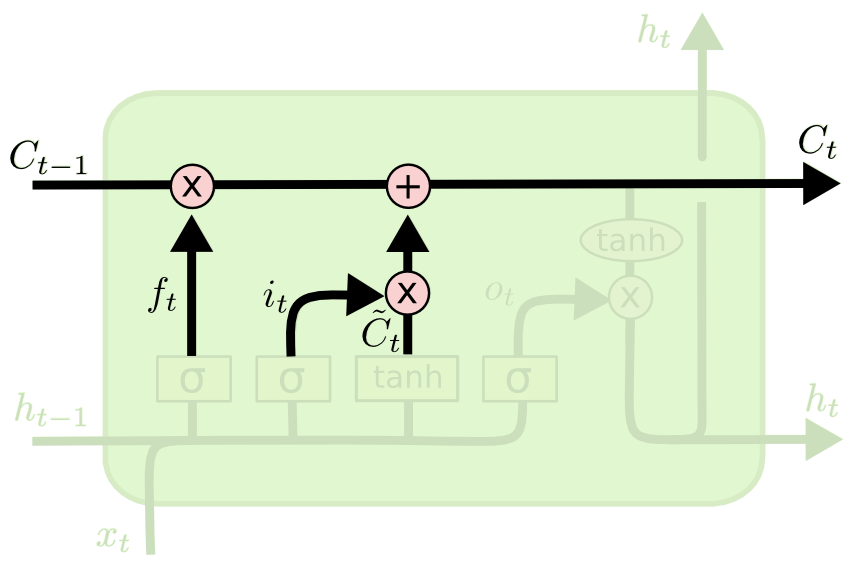
\includegraphics[width=0.45\textwidth]{pictures/LSTM3-focus-C_cut.png}
  \end{center}
  \vspace{-20pt}
  \caption[LSTM: Zellzustands Update]{Zellzustands Update (Quelle: \cite{OlahImg})}
\vspace{-10pt}
\end{wrapfigure}
Nachdem das Forget Gate und das Eingangsgate entschieden haben was mit den Daten passieren soll, wird der Zellzustand aktualisiert. Daf"ur wird der alte Zellzustand C\textsubscript{t-1} mit dem Ergebnis f\textsubscript{t} des Forget Gates multipliziert und somit alles gel"oscht, das vergessen werden soll. Anschlie{\ss}end werden die vom Eingangsgate skalierten und von der tanh-Funktion vorbereiteten Daten zum Zellzustand addiert.

\subsubsection{Ausgabe}
\begin{wrapfigure}{r}{0.45\textwidth}
  \vspace{-30pt}
  \begin{center}
    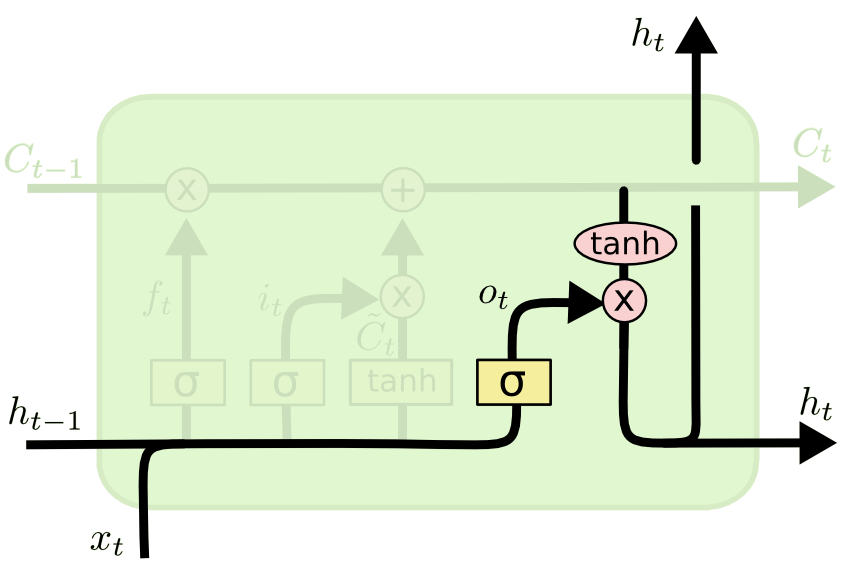
\includegraphics[width=0.45\textwidth]{pictures/LSTM3-focus-o_cut.png}
  \end{center}
  \vspace{-20pt}
  \caption[LSTM: Ausgabe]{Ausgabe (Quelle: \cite{OlahImg})}
\vspace{-10pt}
\end{wrapfigure}
Die Ausgabe erfolgt mit Hilfe eines Ausgabegates, welches ebenfalls eine Sigmoid-Funktion ist. Der Zellzustand wird durch eine tanh-Funktion geleitet und anschlie{\ss}end mit dem Ergebnis der Sigmoid-Funktion multipliziert. Die tanh-Funktion wandelt die Werte in einen Bereich von -1 bis 1 um, welches der typische Wertebereich von KNN-Ausg"angen ist. Durch die Multiplikation kontrolliert das Ausgangsgate, ob und wie stark das Ergebnis ausgegeben wird.

\subsubsection{Zusammenfassung}
Eine Speicherstelle besteht aus einem Zellzustand, der als Ged"achtnis fungiert und drei Gates, die den Zellzustand besch"utzen und kontrollieren. Jedes Gate arbeitet mit einer Sigmoid-Funktion, die einen Wertebereich zwischen 0 und 1 ausgibt und damit die Itensit"at der Aktion bestimmt. Das Forget Gate ist f"ur das L"oschen zust"andig, das Eingangsgate "ubernimmt die Aktion das Neu-Merkens indem es neue Informationen in den Zellzustand speichert und das Ausgangsgate bestimmt die Informationen die ausgegeben werden.


\subsection{LSTM Varianten}
Nicht alle LSTM sind so aufgebaut wie bisher beschrieben. Es gibt viele durch kleine Ver"anderungen leicht abweichende Versionen. Da eine komplette Auflistung den Umfang dieser Arbeit sprengen w"urden, werden hier nur zwei Varianten vorgestellt um einen Eindruck zu vermitteln, welche M"oglichkeiten es gibt.

\subsubsection{Guckl"ocher}
\begin{wrapfigure}{r}{0.35\textwidth}
  \vspace{-40pt}
  \begin{center}
    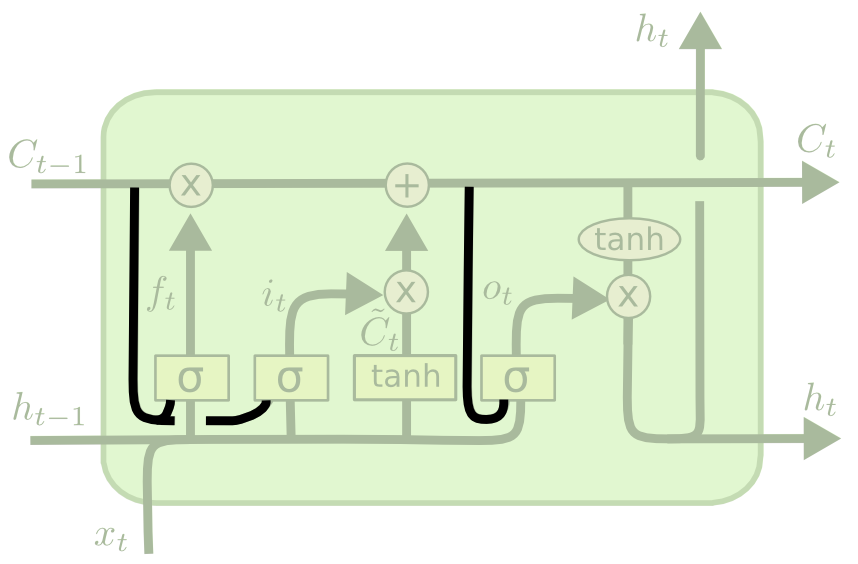
\includegraphics[width=0.35\textwidth]{pictures/LSTM3-var-peepholes_cut.png}
  \end{center}
  \vspace{-20pt}
  \caption[LSTM Variante: Guckl"ocher]{Variante Guckl"ocher (Quelle: \cite{OlahImg})}
\vspace{-10pt}
\end{wrapfigure}
In dieser Variante werden den Gates eine Guckloch-Verbindung hinzugef"ugt. Dies erm"oglicht es den Gates einen Einblick in den aktuellen Zellzustand zu nehmen und die dadurch gewonnenen Informationen in ihre Entscheidung einflie{\ss}en zu lassen. Abbildung 2.11 zeigt diese Verbindungen f"ur alle drei Gates, jedoch ist dies nicht zwingend notwendig. Es besteht die M"oglichkeit auch nur einem oder zwei Gates diese Verbindung zu geben.

\subsubsection{Zusammengef"uhrte Gates}
\begin{wrapfigure}{r}{0.35\textwidth}
  \vspace{-40pt}
  \begin{center}
    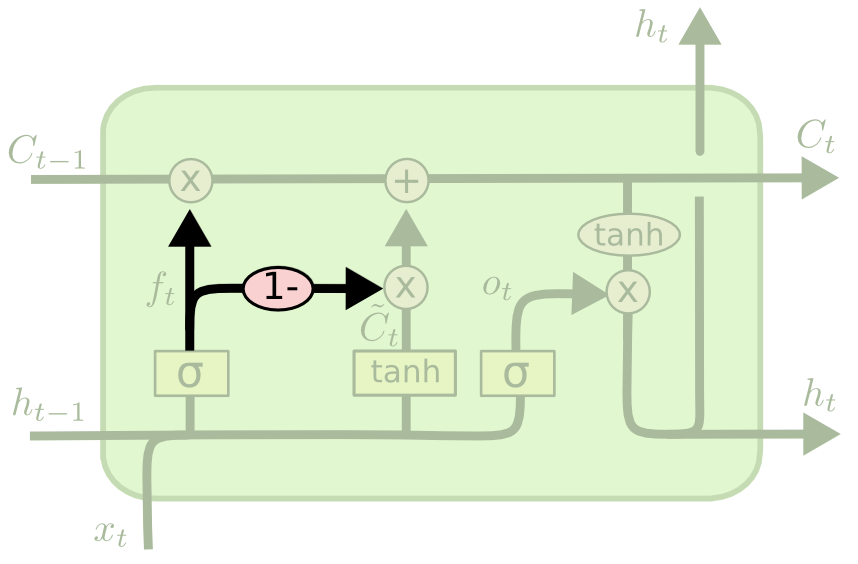
\includegraphics[width=0.35\textwidth]{pictures/LSTM3-var-tied_cut.png}
  \end{center}
  \vspace{-20pt}
  \caption[LSTM Variante: Zusammengef"uhrte Gates]{Variante Zusammengef"uhrte Gates (Quelle: \cite{OlahImg})}
\vspace{-10pt}
\end{wrapfigure}
Eine andere Variante ist in Abbildung 2.12 dargestellt und schlie{\ss}t das Forget Gate und das Eingangsgate zu einem Gate zusammen. Diese Ver"anderung hat die Auswirkung, dass die Entscheidung was gel"oscht und was neu gespeichert wird nur noch gemeinsam getroffen werden kann. Somit kann nur etwas vergessen werden, wenn es durch neue Informationen ersetzt wird und im Umkehrschluss k"onnen neue Informationen nur gespeichert werden, wenn andere Informationen aus dem Zellzustand gel"oscht werden.


\section{Aktueller Forschungsstand}
Long Short-Term Memory Netzwerke wurden von Sepp Hochreiter und J"urgen Schmidhuber Mitte der 90er Jahre vorgestellt und haben seitdem immer mehr an Bedeutung im Bereich des maschinellen Lernens gewonnen. In diesem Abschnitt sollen kurz ein paar Beispiele aus dem aktuellen Forschungsstand gegeben werden, bez"uglich allgemeiner Verwendungen und speziell der Musikerzeugung mit LSTM-Netzwerken.

\subsection{Allgemeine Forschung}

\subsubsection{Analyse von LSTM-Netz-Varianten}
\cite{SpaceOdyssey} f"uhrten eine Studie durch, in der sie acht LSTM-Varianten miteinander verglichen. Die Varianten wichen je um nur einen Aspekt vom Standart-LSTM-Netzwerk ab, um ihre Auswirkung sichtbar zu machen. Getestet wurden die Netze in drei representativen Aufgaben: Spracherkennung, Handschrifterkennung und Musikmodelierung. Ihre Ergebnisse zeigten, dass keine der Varianten das Standart-LSTM-Netz signifikant verbesserte und dass das Forget Gate und die Ausgangsaktivierungsfunktion die kritischten Komponenten eines Netzes sind.

\subsubsection{LSTM-Netzwerk-basierte Merkmalextraktion}
Die menschliche Aktivit"atserkennung findet in mobilen Anwendungen ihren Nutzen. Fitness und Gesundheitsprogramme auf Smartphones basieren meistens auf dem Ansatz der gleitenden Fensterprozedur und erstellen Aktivit"atshypothesen anhand von aufwendig handgemachten Merkmalen. \cite{Chen} stellen in ihrer Arbeit eine LSTM-Netzwerk-basierte Merkmalextraktion vor, welche getestet an Datens"atzen eine sehr hohe Genauigkeit aufweist und somit als praktikabler Ansatz gilt.

\subsubsection{Sprachgenerierung f"ur gesprochene Dialogsysteme}
Die Sprachgenerierung f"ur gesprochene Dialogsysteme erfolgt zur Zeit haupts"achlich "uber regelbasierte Ans"atze und obwohl diese Systeme robust und zuverl"assig arbeiten, ist ein Gespr"ach auf Grund von h"aufigen Wiederholungen identischer Ausgaben oft eint"onig. \cite{Wen} benutzen f"ur ihren Generator ein LSTM-Netzwerk, mit dem Ziel eine gr"o{\ss}ere Varianz in der Satzbildung zu bekommen. Menschliche Richter stuften dieses System h"oher in Informativit"at und Nat"urlichkeit ein und bevorzugten es gegen"uber anderen Systemen.


\subsection{Musikerzeugung}

\subsubsection{Musiksequenzmodellierung mit LSTM-RBM-Netzwerk}
Das Modell von \cite{Lyu} verbindet die F"ahigkeiten von LSTM-Netzwerken und Restricted Boltzmann Maschinen. W"ahrend das Kurzzeitged"achtnis f"ur das erstellen einer Melodie zust"andig ist, sorgt das Langzeitged"achtnis des LSTM-Netzwerkes f"ur ein stimmiges Gesamtergebnis. Die Restricted Boltzmann Maschine ist f"ur die hochdimensionalen Datenmodellierung verantwortlich. Dieser Ansatz verbessert die Leistungsf"ahigkeit von polyphoner Musiksequenzmodellierung erheblich.

\subsubsection{Googles Magenta}
\cite{Magenta} ist ein Deep Learning Musikprojekt von Google mit dem Ziel unwiderstehliche Musik zu generieren. Es ist in Python geschrieben, benutzt die Open Source Software Tensorflow und arbeitet mit MIDI-Dateien. Seit Juni 2016 steht es als Open Source Projekt zur Verf"ugung und enth"allt zur Zeit die Implementation eines RNN und zweier LSTM-Netzwerke. Magenta kann zu diesem Zeitpunkt einen einzelnen String von Noten generieren. (\cite{Asimov})

\subsubsection{BachBot}
\cite{bachbot} ist ein Open Source Forschungsprojekt der Universit"at von Cambridge, dessen Ziel es ist Musikst"ucke zu erzeugen, die von Bachs Werken nicht zu unterscheiden sind. Die Webseite bietet einen Test an, bei dem man sich zwei Musiksequenzen anh"oren und dann raten kann, bei welchen es sich um ein Original von Bach handelt. Dieses Projekt ist in Python geschrieben, benutzt LSTM-Netzwerke und arbeitet mit wav-Dateien.

\subsubsection{GRUV}
\cite{GRUV} ist eine Forschungsarbeit der Universit"at Stanford von \cite{GruvPaper}, welche LSTM-Netzwerke und Gated Recurrent Unit (GRU) Netzwerke zur algorithmischen Musikgenerierung vergleicht. Das Fazit der Autoren lautet, dass die Ausgabe des LSTM-Netzwerkes signifikant musikalisch plausibler ist als die Ausgabe des GRU-Netzes. Dieses Projekt ist ebenfalls in Python verfasst und arbeitet mit waveform-Dateien.

} %% Ende Chapter{RNN und LSTM}